%!TEX root = ../thesis.tex
% ******************************* Thesis Appendix B ********************************

\chapter{Additional information to Chapter 4} \label{appendix:CTsub}
This Appendix contains supplementary figures for Chapter~\ref{chap:CT_bio}.


\section{Supplementary Figures}
\label{sectionB1.1}

\begin{figure}[ht!] 
\centering    
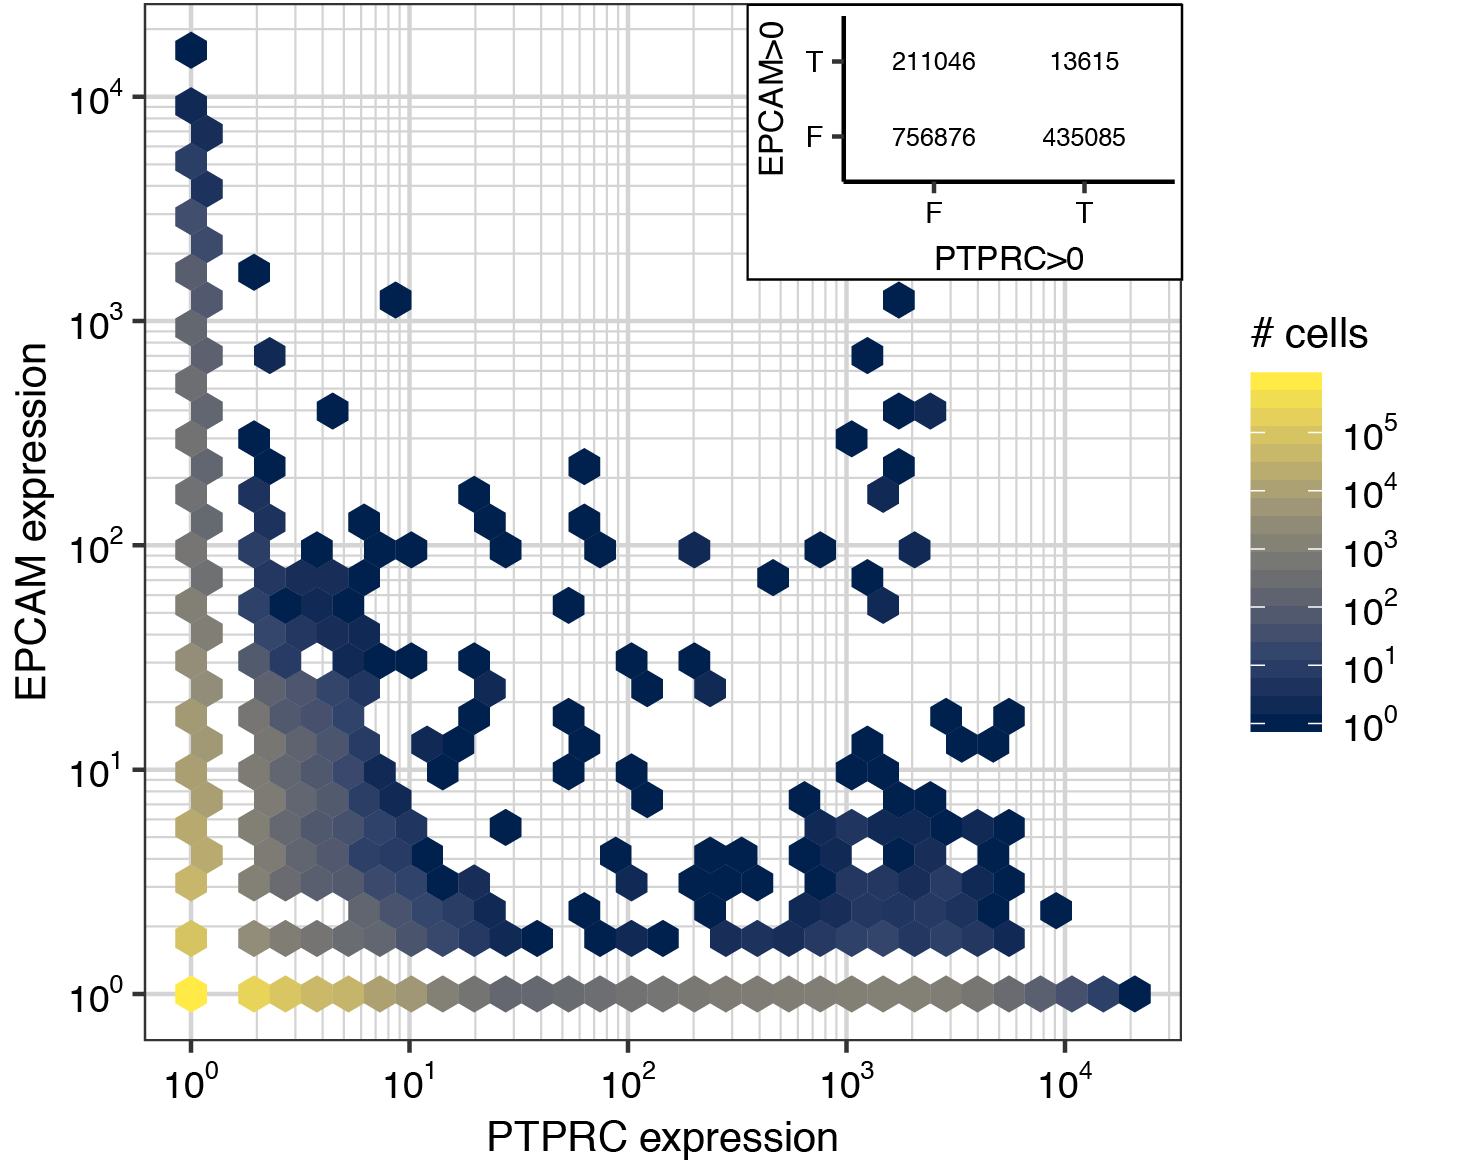
\includegraphics[width=1.0\textwidth]{Appendix2/Figs/PTPRC_EPCAM_human.png} % change word in curlies to change figure
\caption[Expression of \textit{PTPRC} and \textit{EPCAM} in human data collection]{\textbf{Expression of \textit{PTPRC} and \textit{EPCAM} in human data collection (Related to Figure~\ref{fig:chap4_cha})}\newline2D-binned plot of single-cell expression of \textit{PTPRC} (encoding for the CD45 receptor, an immune cell marker), and \textit{EPCAM} (an epithelial cell marker). Inset table (top right) shows the number of cell expressing (T) or not (F) each of the genes. Cells expressing both genes are likely doublets or affected by ambient RNA in droplet-based experiments.}
\label{fig:appB_ptprc}
\end{figure}
